\subsection{\emph{Resultados}}

Para el análisis de la efectividad del método, podemos hacer 3 tipos de
comparaciones:
\begin{enumerate}
	\item Imagen
	\item Histograma
	\item Relación señal-ruido pico ($PSNR$)
\end{enumerate}

\begin{figure*}%
	\centering
		\begin{subfigure}{1.0\columnwidth}
		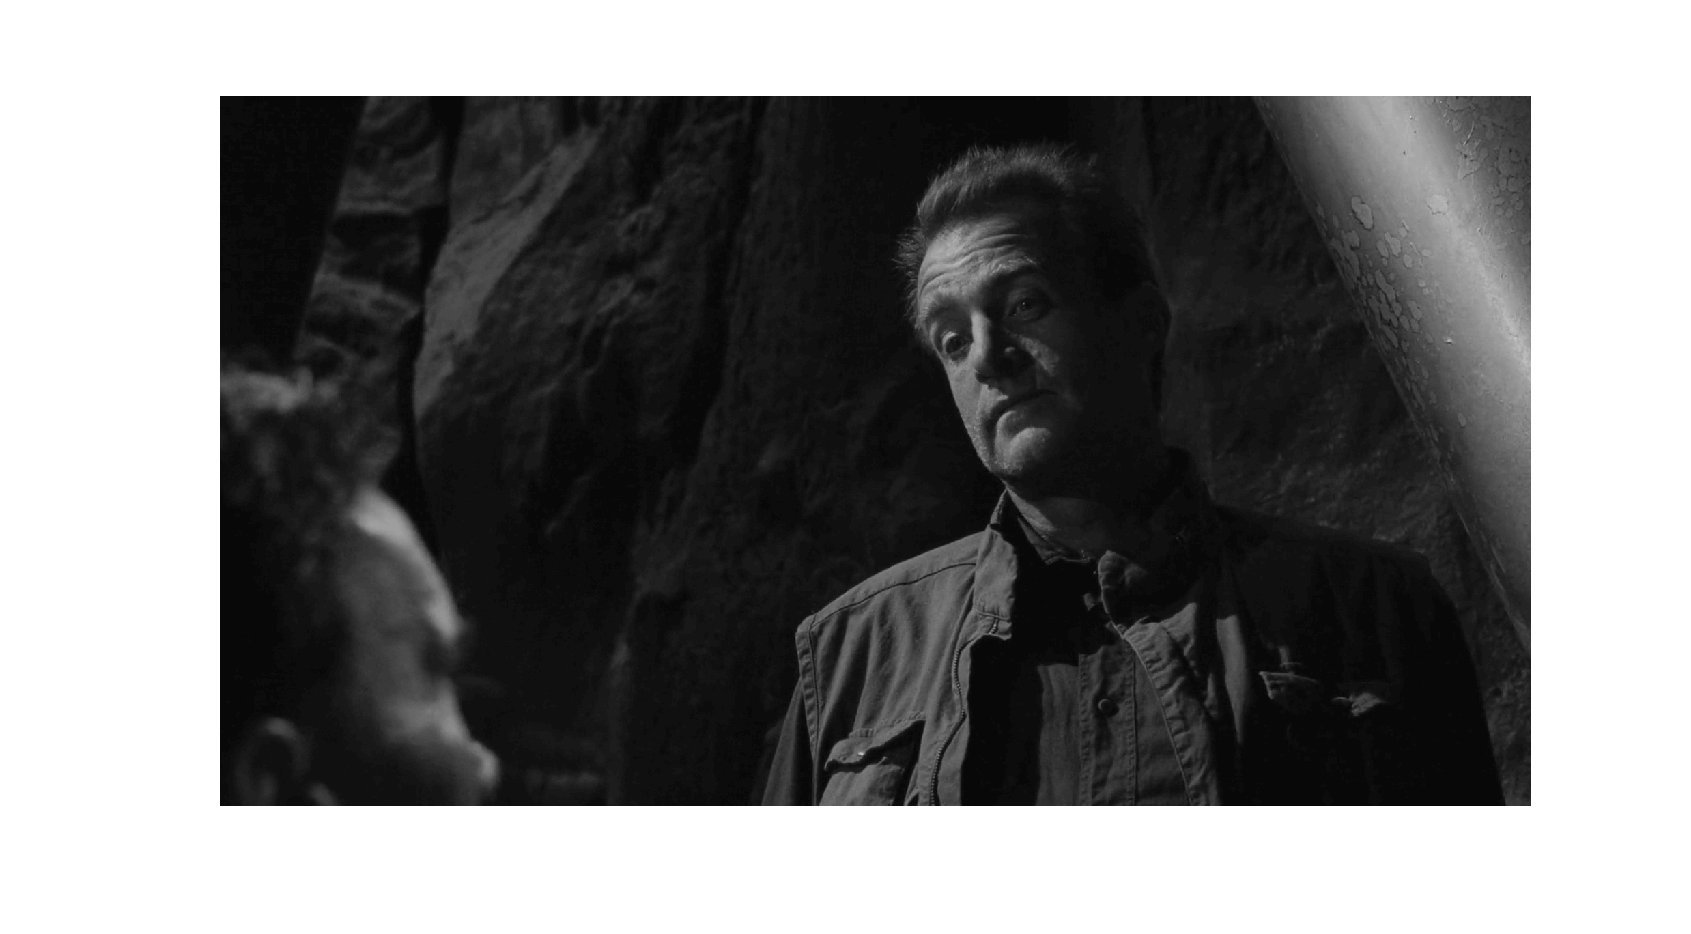
\includegraphics[width=\columnwidth]{result_orig_totalrecall}%
		\caption{Original}%
		\label{subfig:original}%
	\end{subfigure}\hfill%
	\begin{subfigure}{1.0\columnwidth}
		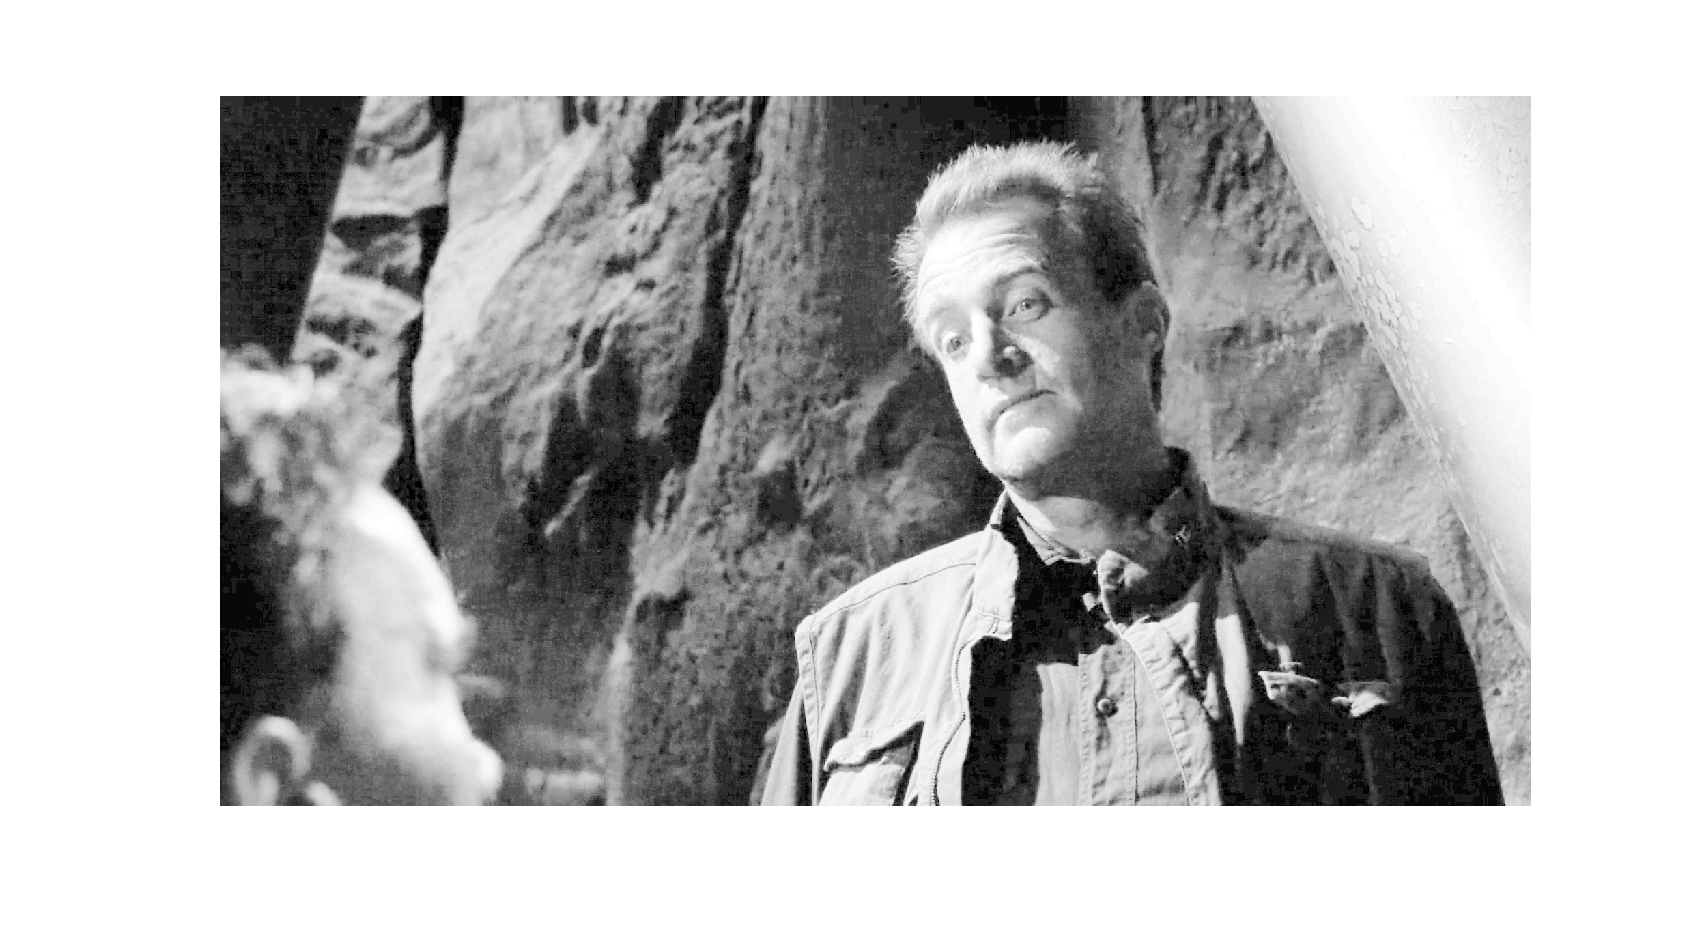
\includegraphics[width=\columnwidth]{result_he_totalrecall}%
		\caption{HE}%
		\label{subfig:he}%
	\end{subfigure}\hfill%
	\begin{subfigure}{1.0\columnwidth}
		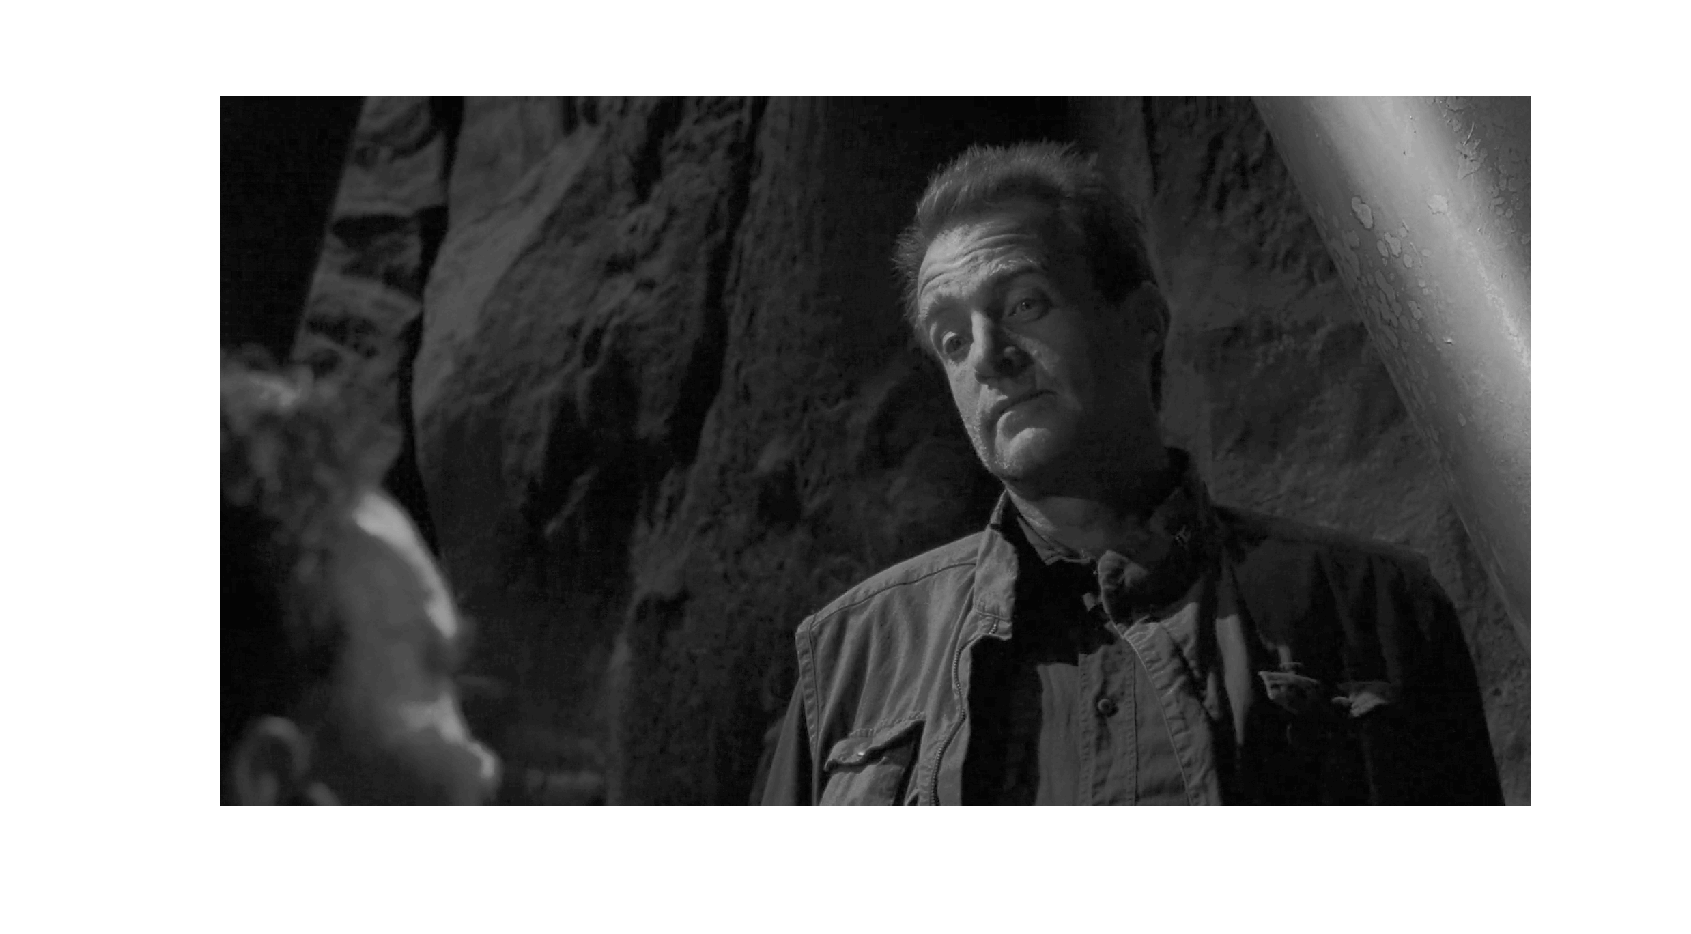
\includegraphics[width=\columnwidth]{result_ace_totalrecall}%
		\caption{ACE}%
		\label{subfig:ace}%
	\end{subfigure}%
	\caption{Comparación de resultados para la imagen de prueba \emph{Total Recall}.}
	\label{fig:comp_imagenes}
\end{figure*}

Como se puede ver en la Figura \ref{fig:comp_imagenes}, la ecualización del
histograma puede generar imágenes saturadas con respecto a las originales
(con Figura \ref{subfig:he} y Figura \ref{subfig:original} respectivamente). En
cambio, al hacer la comparación de la Figura \ref{subfig:original} y la alterada
por $ACE$ (Figura \ref{subfig:ace}), esta última muestra un mejor contraste
visual versus su contraparte de $HE$.\\

Para evaluar la variación del rango dinámico, se hallan los histogramas
correspondientes para cada caso como se puede ver en la Figura
\ref{fig:comp_histo}.

\graficarMulticolPNG{result_comp_hist}{Histograma de las imágenes procesadas por
HE y ACE, en comparación con la original.}{fig:comp_histo}

Como se puede ver en la Figura \ref{fig:comp_histo}, en ambos casos ($HE$ y
$ACE$) el rango dinámico aumenta. Sin embargo, se puede apreciar que el
histograma del $HE$, aunque de  mayor rango, contiene mayor cantidad de
discontinuidades o picos, mientras que el del $ACE$ tiene una envolvente más
suave y concentrada en un rango dado. Esto implica que la imagen modificada por
$HE$ presenta mayores saturaciones, resultando en artefactos indeseados.

Finalmente, en la Tabla \ref{tab:comp_psnr} se hallan los valores de $PSNR$ de
los dos métodos bajo análisis. Queda en evidencia de forma analítica, que
la propuesta de $ACE$ mejora la imagen en mayor medida que el $HE$, al tener un
$PSNR$ mayor en todos los casos. Para la imagen \emph{Shadowlands}, el $MSE$
utilizado para el cálculo de $PSNR$ es tan pequeño que genera un resultado infinito.\\

\noindent
\begin{minipage}{\columnwidth}
	\makeatletter
	\newcommand{\@captype}{table}
	\centering
	\begin{tabular}{@{}ccc@{}}
		\toprule
		Imagen de prueba& ${PSNR}_{he}$ & ${PSNR}_{ace}$ \\
		\midrule
		Total Recall	& $54.524$      & $59.705$       \\
		Shadowlands  	& $\infty$      & $\infty$       \\
		Odín         	& $28.232$      & $32.429$		 \\
		\bottomrule
	\end{tabular}
	\caption{\emph{Peak Signal-to-noise ratio} para las 3 imágenes de prueba}
	\label{tab:comp_psnr}
\end{minipage}

